% Kelvin / DtN open-boundary solve -- FLOWCHART (TikZ shapes.geometric idiom).
% Recipe: radia_mcp.figure  figure_diagram_recipes(topic="tikz_flowchart").
% Build:  pdflatex kelvin_dtn_solve_flowchart.tex   (standalone -> PDF, embed at column width)
\documentclass[tikz,border=2mm]{standalone}
\usepackage{newtxtext,newtxmath}                 % match IEEE/IEEJ body font
\usetikzlibrary{shapes.geometric, shapes.misc, arrows.meta, positioning}  % shapes.misc = rounded rectangle
\begin{document}
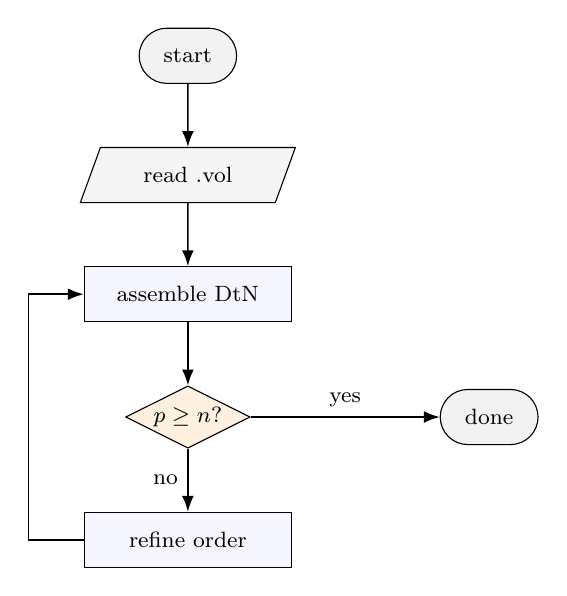
\begin{tikzpicture}[
  node distance=8mm and 14mm, font=\footnotesize,
  start/.style   ={rounded rectangle, draw, fill=black!5, minimum height=7mm, inner xsep=3mm},
  process/.style ={rectangle, draw, fill=blue!4,  minimum height=7mm, text width=24mm, align=center},
  decision/.style={diamond, draw, fill=orange!12, aspect=2, inner sep=1pt, align=center},
  io/.style      ={trapezium, trapezium left angle=70, trapezium right angle=110,
                   draw, fill=black!4, minimum height=7mm},
  arrow/.style   ={-{Latex[length=2mm]}, semithick},
]
  \node[start]                    (a) {start};
  \node[io,       below=of a]     (b) {read .vol};
  \node[process,  below=of b]     (c) {assemble DtN};
  \node[decision, below=of c]     (d) {$p\ge n$?};
  \node[process,  below=of d]     (e) {refine order};
  \node[start,    right=24mm of d](f) {done};
  \draw[arrow] (a)--(b); \draw[arrow] (b)--(c); \draw[arrow] (c)--(d);
  \draw[arrow] (d)-- node[left]{no} (e);
  \draw[arrow] (e.west) -- ++(-7mm,0) |- (c.west);     % feedback loop, routed orthogonally
  \draw[arrow] (d)-- node[above]{yes} (f);
\end{tikzpicture}
\end{document}
